\documentclass[../main]{subfiles}
\begin{document}
\setcounter{secnumdepth}{3}
    \chapter{実験}
    \section{実験目的}
        本研究で提案した全天球カメラ画像に基づく通路分類手法の有効性をロボットを用いた実環境での実験により検証する.
    \section{実験の概要}
        提案した通路分類手法の有効性をロボットを用いた実環境での実験により検証する.
        実験環境は\fref{figure::3floor_map}に示す千葉工業大学津田沼キャンパス2号館3階の廊下とした.
        \begin{figure}[H]
         \centering
         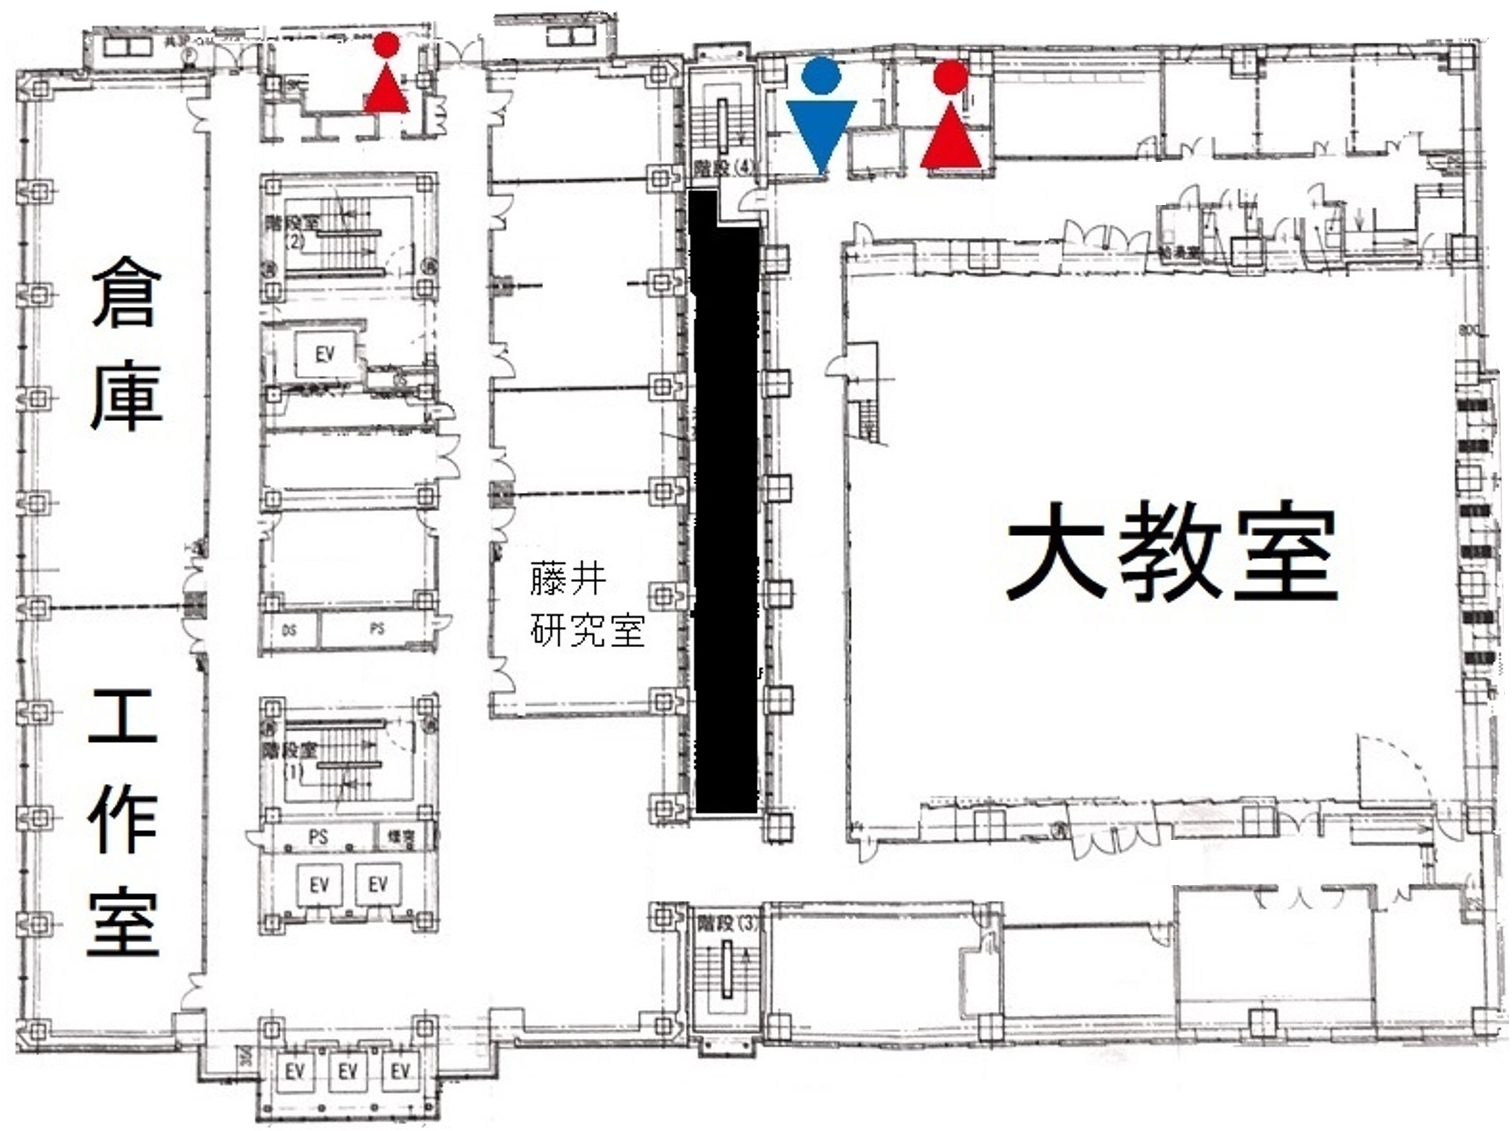
\includegraphics[width=10cm]{../images/MAP_Tsudanuma2-3.png}
         \caption{Experiment environment}
         \label{figure::3floor_map}
        \end{figure}

    \section{実験装置}
        実験には本研究室で開発をしているORNE-αを用いた.また,機体とその構成,使用したPCのスペックをそれぞれ
        \fref{figure::robot_image},\tref{table::robot_spec},\tref{table::pc_spec}に示す.

        \begin{figure}[H]
        \centering
        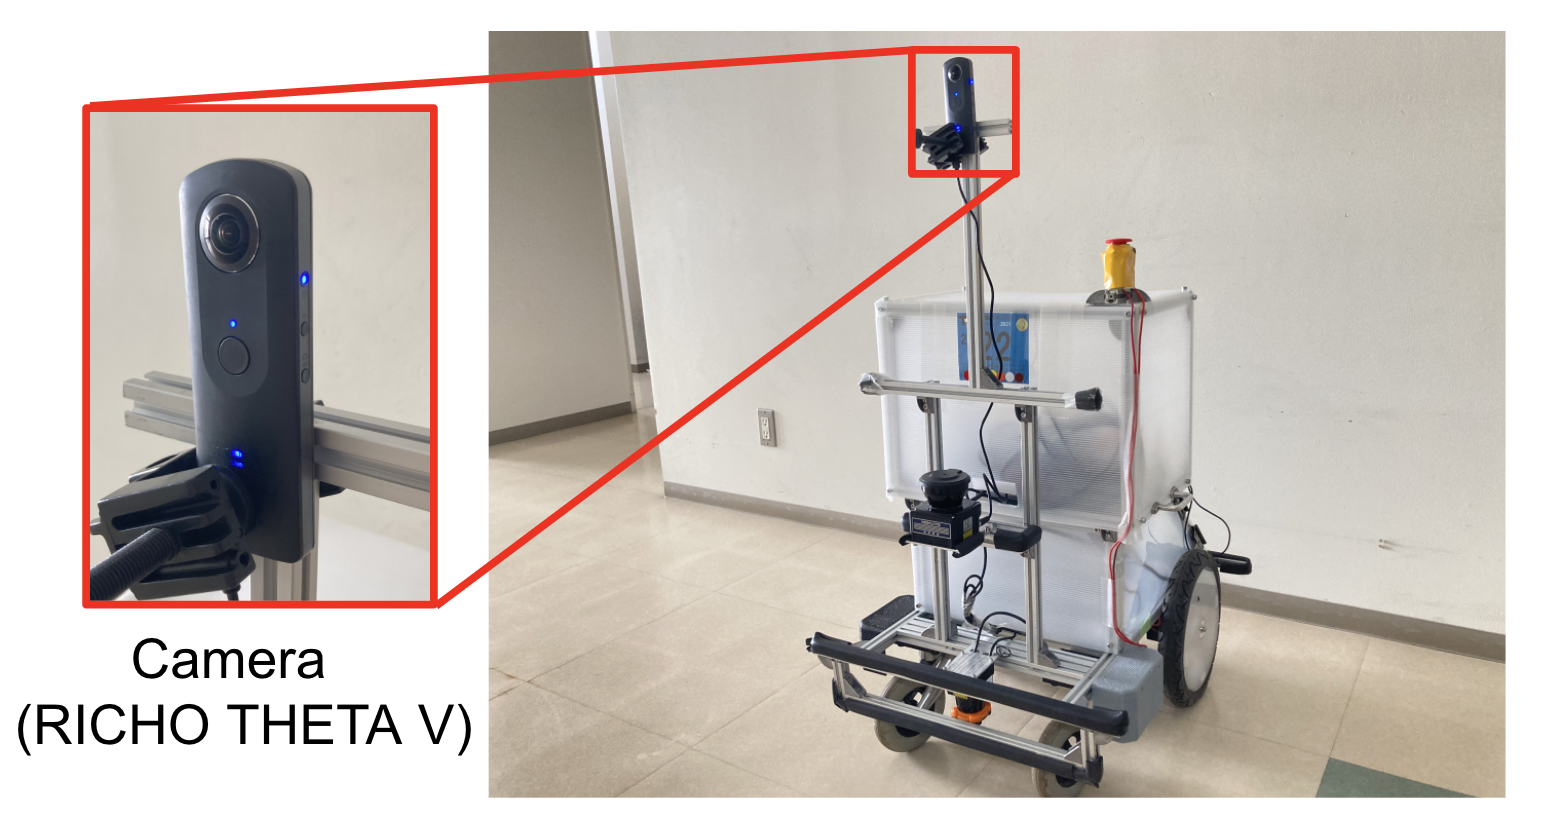
\includegraphics[width=13cm]{../images/experimental_machine_wide.png}
        \caption{ORNE-α}
        \label{figure::robot_image}
        \end{figure}

        \begin{table}[H]
         \centering
         \caption{Specification of PC}
         \begin{tabular}{l|l} \hline
         \multicolumn{1}{c|}{CPU} & \multicolumn{1}{c}{Core i7-9750H(Intel)} \\ \hline
         \multicolumn{1}{c|}{RAM} & \multicolumn{1}{c}{16GB} \\ \hline
         \multicolumn{1}{c|}{GPU} & \multicolumn{1}{c}{RTX 2070 Max-Q} \\ \hline
         \end{tabular}
         \label{table::pc_spec}
        \end{table}

        \begin{table}[H]
            \centering
            \caption{Specification of ORNE-α}
            \begin{tabular}{l|l}\hline
            \multicolumn{1}{c|}{item}                                                              & \multicolumn{1}{c}{ORNE-α}                              \\ \hline
            \multicolumn{1}{c|}{Depth{[}mm{]}}                                                     & \multicolumn{1}{c}{710} \\ \hline
            \multicolumn{1}{c|}{Wide{[}mm{]}}                                                      & \multicolumn{1}{c}{560}                                 \\ \hline
            \multicolumn{1}{c|}{Height{[}mm{]}}                                                    & \multicolumn{1}{c}{810}                                  \\ \hline
            \multicolumn{1}{c|}{Weight{[}kg{]}}                                                    & \multicolumn{1}{c}{20}                                   \\ \hline
            \multicolumn{1}{c|}{\begin{tabular}[c]{@{}c@{}}Wheel diameter\\ {[}mm{]}\end{tabular}} & \multicolumn{1}{c}{304}                                   \\ \hline
            \multicolumn{1}{c|}{Battery}                                                           & \multicolumn{1}{c}{LONG WP12-12 × 2}                      \\ \hline
            \multicolumn{1}{c|}{Motor}                                                             & \multicolumn{1}{c}{Oriental motor TF-M30-24-3500-G15L/R}  \\ \hline
            \multicolumn{1}{c|}{Spherical camera}                                                  & \multicolumn{1}{c}{RICOH THETA V}  \\ \hline
            \end{tabular}
            \label{table::robot_spec}
            \end{table}

    \clearpage

    \section{全天球カメラを用いた通路分類の検証}
        \subsection{実験方法}
        全天球カメラを取り付けたロボットを\fref{figure::experiment_point}の丸の図形で示す25箇所に配置し,
        各地点で全天球カメラの画像データを取得する.そして,提案手法を用いてそれらの画像から通路の特徴分類ができるかどうかを検証する.
        \fref{figure::experiment_point}の赤,緑,オレンジ,青の丸は各地点の通路の特徴を表しており,それぞれ三叉路,角,一本道,突き当たりである.
        また,三叉路と角の箇所では通路に侵入する際の向きにより\fref{figure::experiment1}のように各通路方向に特徴が変化する.
        そのため,それらの箇所ではロボットの向きを変え,同一箇所でも複数の画像データをキャプチャして検証する.
        本実験では,25箇所・47の画像データで検証を行った.

        \begin{figure}[H]
         \centering
         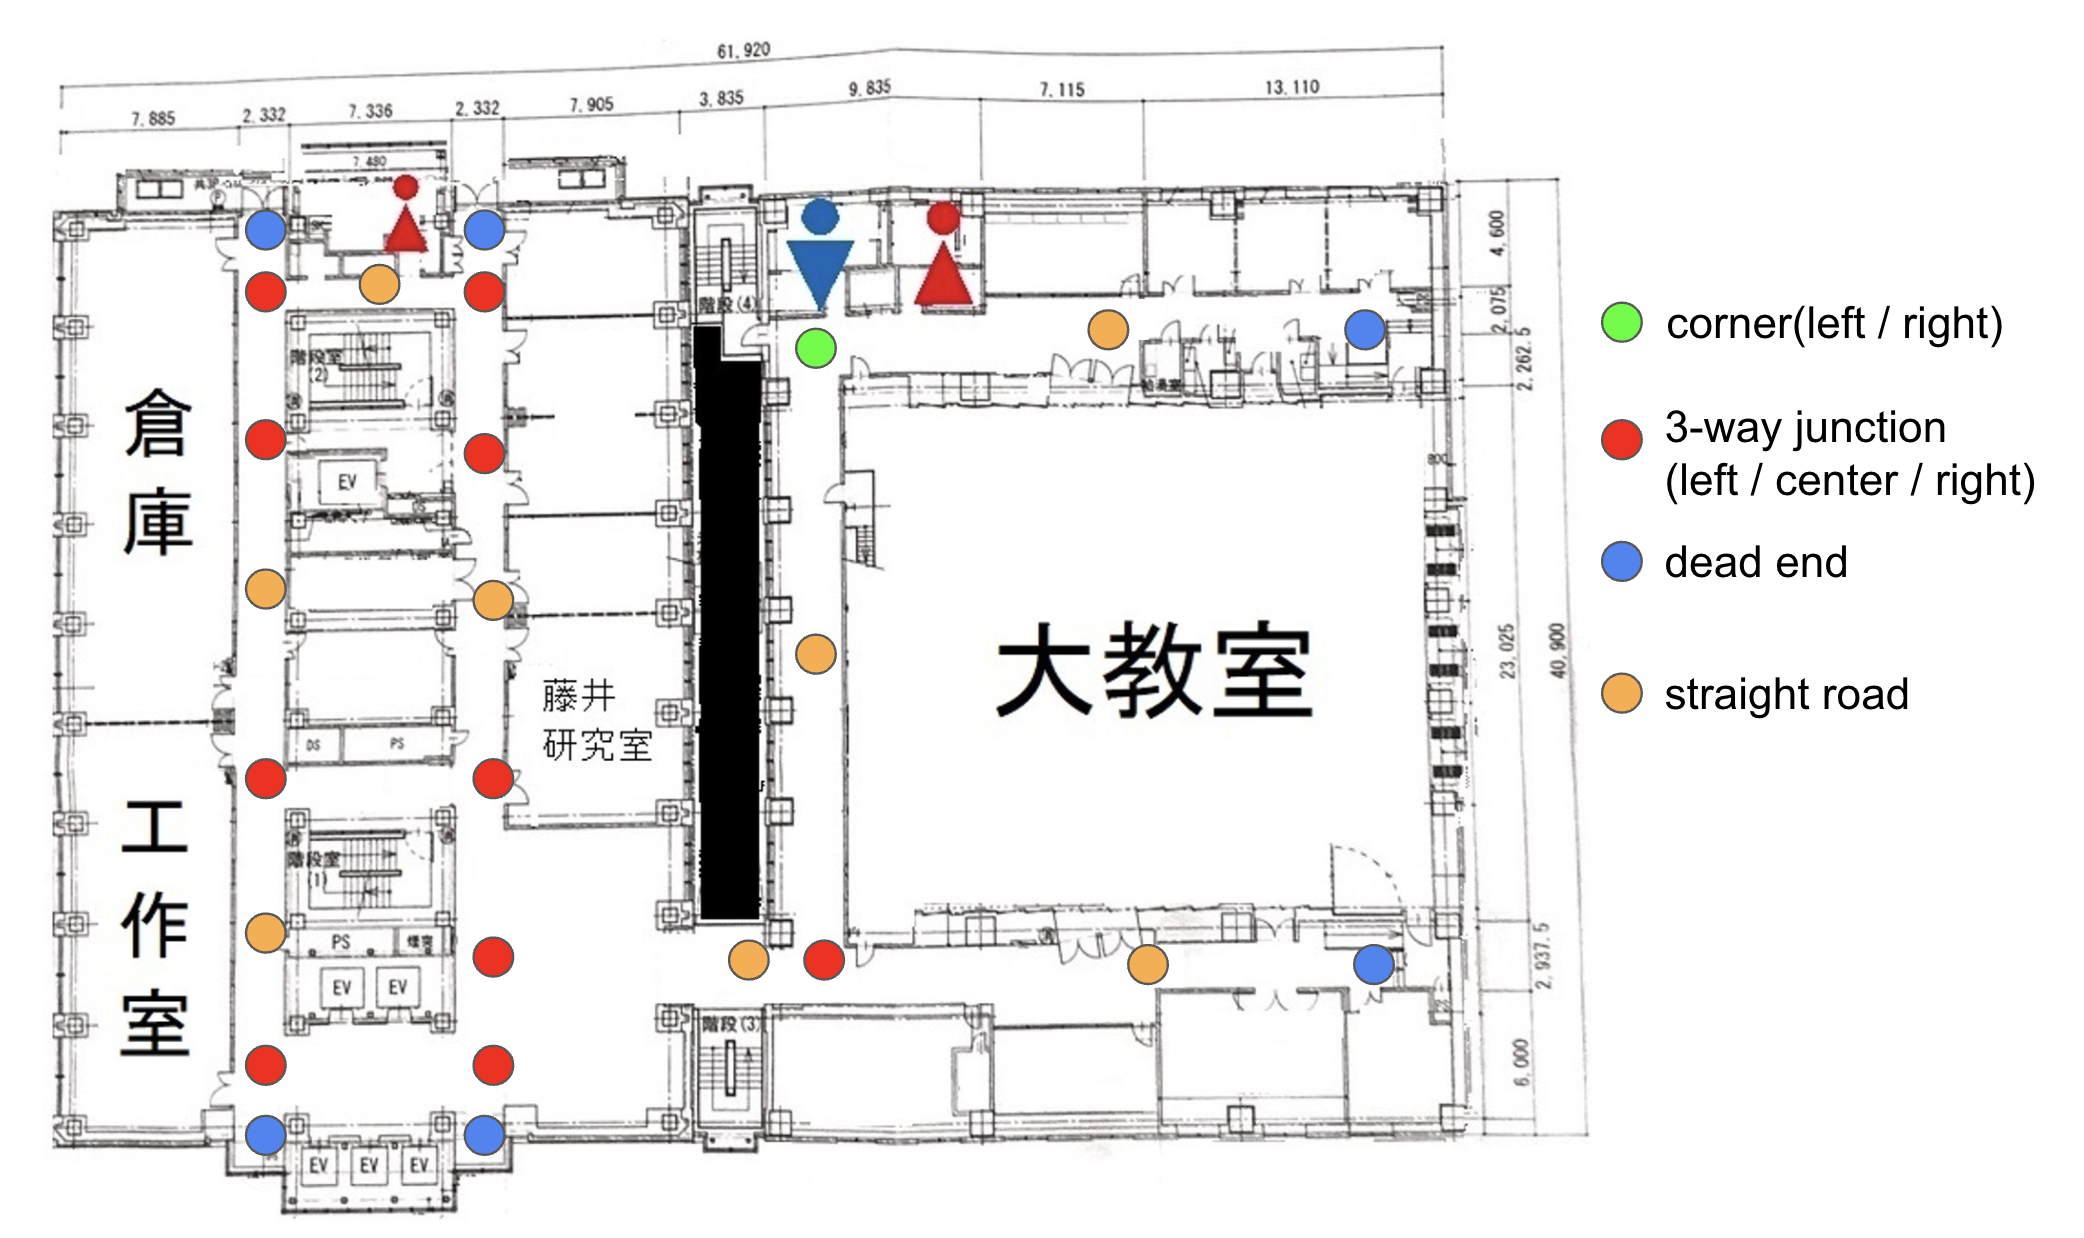
\includegraphics[width=14cm]{../images/experiment_point.png}
         \caption{25 places to place robots in aisle classification experiments}
         \label{figure::experiment_point}
        \end{figure}

        \begin{figure}[H]
         \centering
         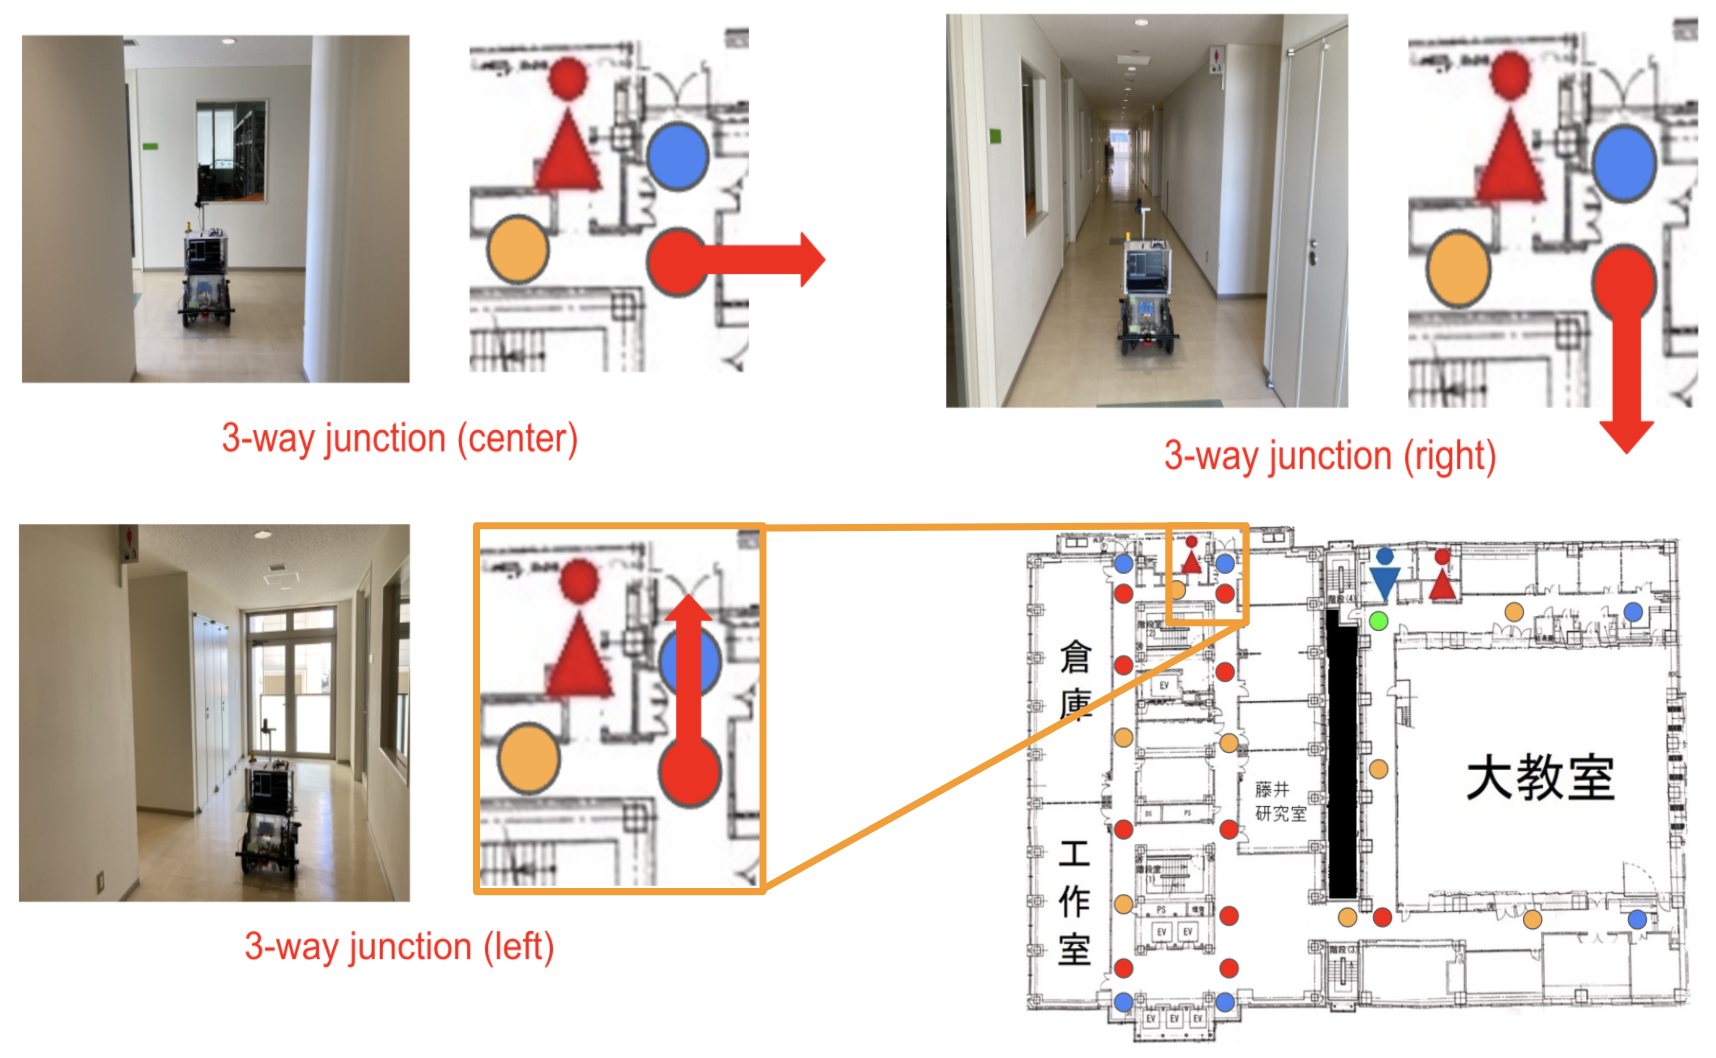
\includegraphics[scale=0.35]{../images/robot_direction.png}
         \caption{Relationship between the arrow in the map and the orientation of the robot}
         \label{figure::experiment1}
        \end{figure}

        \newpage

        \subsection{結果と考察}
        実験の結果,47の画像データ中42を正しく分類できることが確認できた.
        通路の分類に成功した箇所とその地点での検出器による物体検出の結果を\fref{fugure::success_img}に示す.
        成功した例では各画像データから検出器により物体検出が正しく行われており,通路の方向に基づき通路の分類ができていることを確認できた.
        一方,分類に失敗した箇所は\fref{figure::experiment_result}に示す3箇所・5の画像データである.また,各矢印はロボットの向きを示す.
        失敗の原因は以下の通りで, 全て検出器での誤検出が原因であった. \\
        ・1:検出器による後方通路の検出失敗\\
        ・2:検出器により通路を突き当たりと誤検出で正しく通路の特徴を分類することができた.

        本実験により,検出器による物体検出が正しく行われた場合,通路の分類を正しく行えることがわかった.
        また,検出器による誤検出は,通路と突き当たりの境界が曖昧であることが原因で発生したと考えられる.
        突き当たり

        % \begin{figure}
        %     \centering
        %     \includegraphics{}
        %     \caption{}
        %     \label{figure::success_img}
        % \end{figure}


        % \begin{figure}[H]
        %     \centering
        %     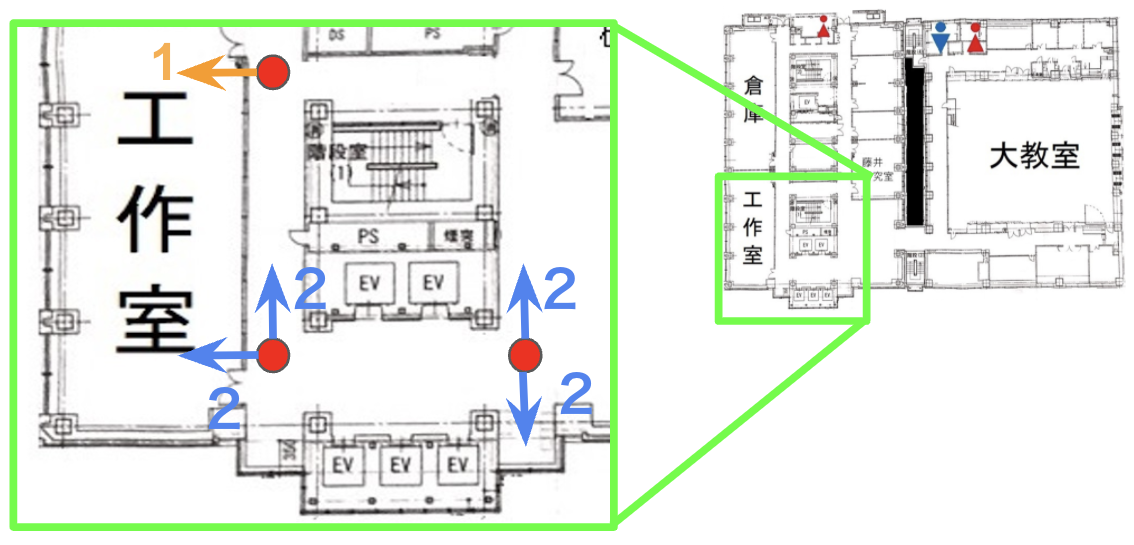
\includegraphics[scale=0.5]{../images/experiment_result}
        %     \caption{Points where passage classification failed}
        %     \label{figure::experiment_result}
        % \end{figure}
\end{document}